\documentclass[a4paper,10pt]{article}
\usepackage[utf8]{inputenc}
\usepackage{listings}
\usepackage{graphicx}

\title{Rechnernetze Aufgabe 3 Konzept}

\author{
  Triebe, Marian\\
  \texttt{marian.triebe@haw-hamburg.de}
  \and
  Kirstein, Katja\\
  \texttt{katja.kirstein@haw-hamburg.de}
}

\begin{document}

\maketitle

\section{Aufgabenbeschreibung}
\begin{figure}[h]
  \centering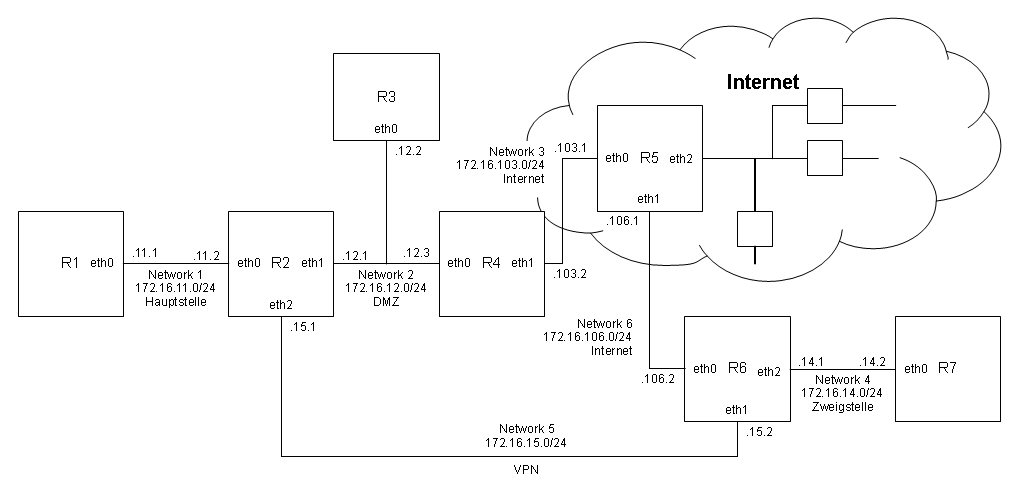
\includegraphics[scale=.35]{topo.jpg}
  \caption{Netzwerk Topologie [1]}
\end{figure}
Es soll ein Netzwerk eingerichtet werden, welches aus verschiedenen Subnetzwerken besteht. Zugriff zwischen den
einzelnen Netzen soll theoretisch erlaubt sein, hierzu muss das Routing in die verschiedenen Netzwerke konfiguriert werden.
Desweiteren sind Firewalls der einzelnen Router einzustellen, so dass nur folgende Pakete geroutet werden:
\begin{itemize}
 \item Ping zwischen allen Computern im internen Netz sowie ins Internet, kein Ping vom Internet aus
 \item SSH von den internen Hosts (R1, R7) auf R3, R3 kein SSH Zugriff auf interne Hosts. Daten müssen über das VPN laufen.
 \item FTP sowie HTTP sollen für R3 freigegeben werden. Dazu ist die stateful Einstellung von iptables zu benutzen.
\end{itemize}
Außerdem soll R7 Zugang zum Internet bekommen. Dies soll durch ein NAT realisiert werden. Dazu muss R6 entsprechend eingestellt werden.

\section{Routing}
Diese Netzwerke müssen beim routing eingestellt werden:\newline
\begin{itemize}
 \item Wenn R1 auf andere Netzwerke zugreifen will, geschiet dies über den R2. 
 \item R2 kommt in andere Netzwerke über R6, ggf. R4 wenn es das Internet ist.
 \item R3 gelangtin andere Netzwerke über R2 und R4.
 \item R4 geht in andere Netzwerke über R2 und R5.
 \item R5 kann übet R4 und R6 auf die anderen Netzwerke zugreifen.
 \item R6 geht über R5 oder R2. um in andere Netzwerke zu gelangen.
 \item R7 muss über R6 gehen.
\end{itemize}

\section{iptables Konzept}
Die Policy für die Netzwerke ist drop. Alle nicht explizit zugelassenen Pakete werden nicht durchgelassen.
Ping, SSH, FTP sowie HTTP sollen teilweise erlaubt sein. Hierzu kann eine stateful Firewall verwendet werden.

\section{Quellen}
[1] http://tiserver02.cpt.haw-hamburg.de/htm/rn.php?page=aufgabe3

\end{document}